% Title Page

\backgroundsetup{%
    contents={%
        \begin{tikzpicture}
            %\pgfmathsetmacro{\myopacity}{mod(\thepage-1,4)*0.25+0.25}
            \node[opacity=0.35] {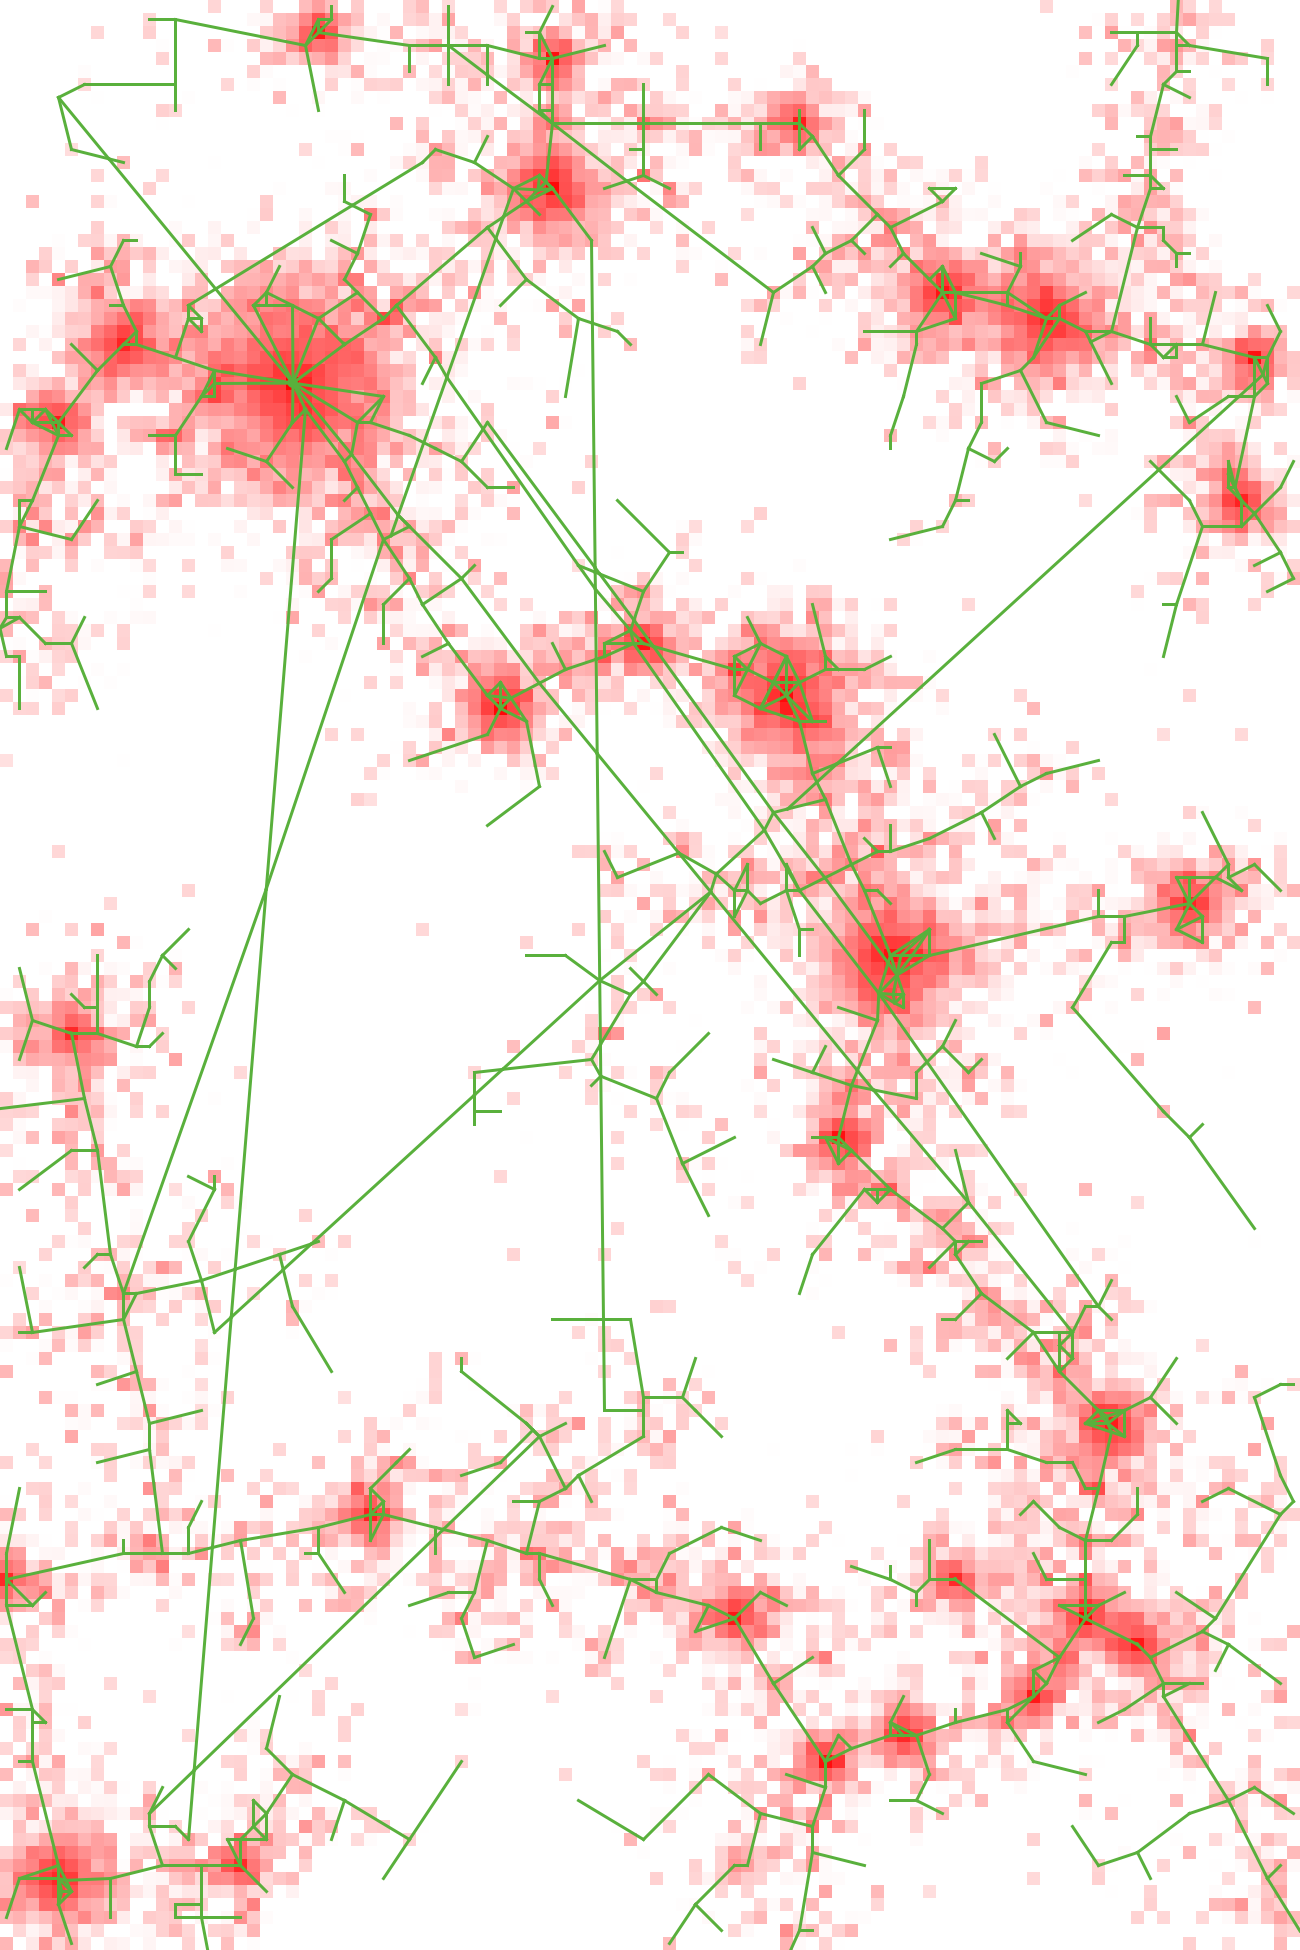
\includegraphics[width=\paperwidth]{Figures/Cover/cover2}};
        \end{tikzpicture}
    }
}


\begin{titlepage}

%\newgeometry{bottom=1cm}

\begin{addmargin}[-1cm]{-3cm}
\begin{center}
\large

\hfill


\vspace{-1.5cm}

\includegraphics[width=5cm]{Figures/Art/logouspc.png}
\hfill

\includegraphics[height=4cm]{Figures/Art/Logo-P7.png}

\vspace{0.5cm}

\begingroup
\bpar{
\spacedallcaps{PhD Thesis}\\\medskip
\spacedallcaps{from Université Sorbonne Paris Cité}\\\medskip
\spacedallcaps{Prepared at Université Paris Diderot}\\\medskip
\spacedallcaps{École Doctorale de Géographie de Paris (ED 434)}\\\vspace{0.5cm}
\textit{UMR CNRS 8504 Géographie-cités / Équipe P.A.R.I.S.}\\
\textit{UMR-T IFSTTAR 9403 LVMT}
}{
\spacedallcaps{Thèse de Doctorat}\\\medskip
\spacedallcaps{de l'Université Sorbonne Paris Cité}\\\medskip
\spacedallcaps{Préparée à l'Université Paris Diderot}\\\medskip
\spacedallcaps{École Doctorale de Géographie de Paris (ED 434)}\\\vspace{0.5cm}
\textit{UMR CNRS 8504 Géographie-cités / Équipe P.A.R.I.S.}\\
\textit{UMR-T IFSTTAR 9403 LVMT}
}
\endgroup



\vspace{1.5cm}

\begingroup
%\color{Maroon}
\textbf{\spacedallcaps{\myTitle}} \\ \bigskip % Thesis title
\endgroup

\vspace{1.5cm}



% https://tex.stackexchange.com/questions/229593/gradient-to-transparent-horizontal-for-beamer-frametitle

%\vspace{-2cm}
%{\transparent{0.7} 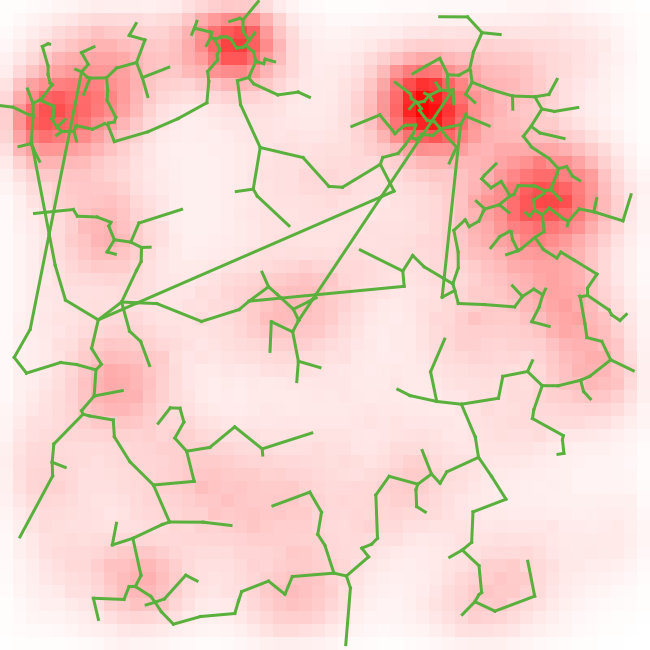
\includegraphics[width=\textwidth]{Figures/Cover/cover}} \\ %\vspace{0.5cm} % Picture
%\vspace{-3cm}

\bpar{
\textit{Presented by} \spacedlowsmallcaps{\myName}\\
}{
\textit{Présentée par} \spacedlowsmallcaps{\myName}\\ % Your name
}
\bigskip

\bpar{
PhD Thesis in Geography
}{
Thèse de doctorat de Géographie
}


%\mySubtitle \\ \medskip % Thesis subtitle
\bpar{
Under the supervision of \myProf and \myOtherProf \\ \medskip
}{
Dirigée par \myProf et \myOtherProf \\ \medskip
}
%\myDegree \\
%\myDepartment \\  \medskip
%\myFaculty \\  \bigskip
%\myUni \\ \bigskip

%\hspace{1.5cm}

%\myTime\ -- \myVersion % Time and version

%\hspace{1.5cm}


\vspace{0.5cm}

\bpar{
\textit{Presented and defended publicly at the Institut des Systèmes Complexes (Paris) on June 11th 2018, with a jury composed by :}
}{
\textit{Présentée et soutenue publiquement à l'Institut des Systèmes Complexes (Paris) le 11 juin 2018, devant le jury composé de :}
}

\bigskip


\begin{adjustwidth*}{-0.5cm}{-2cm}
\begin{minipage}{0.28\linewidth}
\raggedright
\textbf{\noun{Denise Pumain}}\\
\textbf{\noun{Didier Josselin}}\\
\textbf{\noun{Catherine Morency}}\\
\textbf{\noun{Olivier Bonin}}\\
\textbf{\noun{Anne Ruas}}\\
\textbf{\noun{Arnaud Banos}}\\
\textbf{\noun{Florent Le Néchet}}
\end{minipage}
\begin{minipage}{0.7\linewidth}
\raggedright
Professeure, Université Paris 1 (Présidente du Jury)\\
Directeur de Recherche, CNRS (Rapporteur)\\
Professeure, Ecole Polytechnique de Montréal (Rapporteuse)\\
Chargé de Recherche, IFSTTAR (Examinateur)\\
Directrice de Recherche, IFSTTAR (Examinatrice)\\
Directeur de Recherche, CNRS (Directeur)\\
Maître de Conférences, Université Paris-Est (Directeur)\\
\end{minipage}
\end{adjustwidth*}

\vspace{2cm}

\begin{minipage}{0.28\linewidth}
	
\includegraphics[width=\textwidth]{Figures/Art/by-nc-sa.png}
\end{minipage}
\hfill
\begin{minipage}{0.7\linewidth}
This work is licensed under a \href{http://creativecommons.org/licenses/by-nc-sa/4.0/}{Creative Commons Attribution-NonCommercial-ShareAlike 4.0 International License}.
\end{minipage}


\end{center}
\end{addmargin}

\end{titlepage}

%\restoregeometry

\backgroundsetup{%
    contents={}
}


